The setup which is used to meassure the PV systems and to gather data
is very simple.

For the logging of weather information a simple program was used to
query OpenWeatherMap.org for weather information, and logging them
into a database.  When OpenWeatherMap is queried based on GPS
coordinates, the actual weatherstation is selected
non-deterministicly.  Thus for Mønsted (where the solar panels are
located), it actually alternates between two towns (Stoholm and Karup)
for weather data as can be seen on figure \ref{fig:mapsPicture}.

\begin{figure}[h]
  \centering
  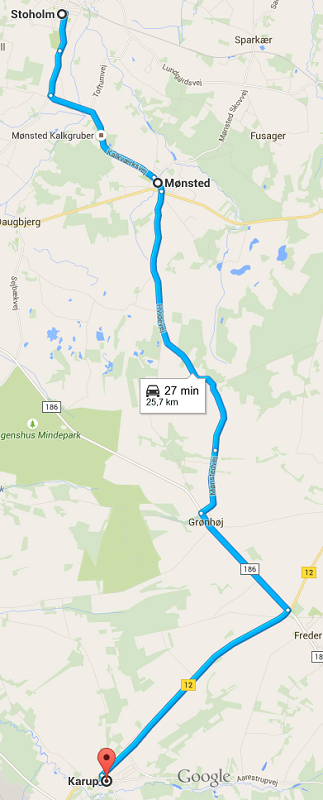
\includegraphics{mapsPicture}
  \caption{3 towns where data is recorded}
  \label{fig:mapsPicture}
\end{figure}

At the PV system the serial interface of the inverter is used.  The
setup is based on a Raspberry PI with an RS485 serial converter to
connect to the inverter.  The setup is described in further detail at
\url{https://code.google.com/p/eversolar-monitor/wiki/Hardware}.  The
scematics can be seen on figure \ref{fig:hardware}.

\begin{figure}[h]
  \centering
  % 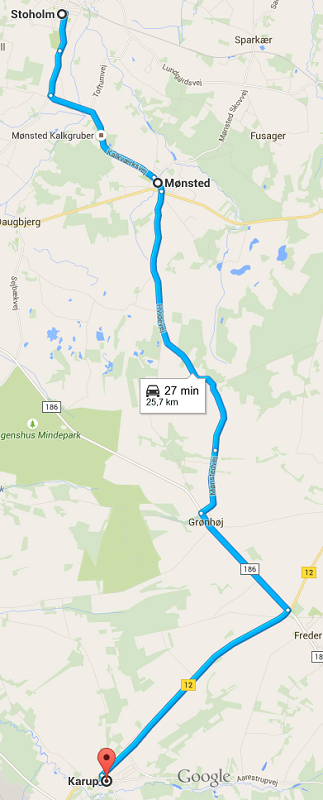
\includegraphics{MapsPicture.png}
  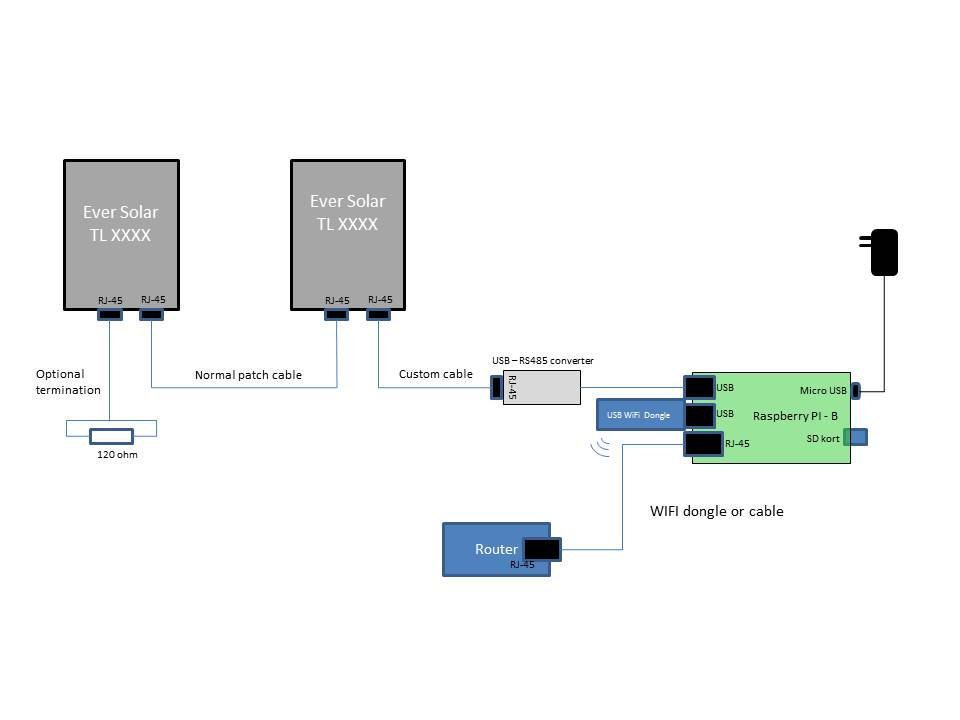
\includegraphics[width=1\textwidth]{hardware}
  \caption{Diagram over the harware setup}
  \label{fig:hardware}
\end{figure}

The data gathered is initially logged at local database, but once
gathered is moved to full database server, normalizing the data, so
they can be compared.  The database is used for more powerful
functions such as dividing the data into intervals and doing simple
statistic caluculations.
D3 is then used to visualize the data, which is a lot easier if the data 
is the same place. Visualizing of the statistic is required to be able to 
see any link between the data.

The source code for the system is freely available on GitHub at
\url{https://github.com/rohdef/EverSolar-reader}, the data and
aggregate functions is available from the PostgreSQL database located
at \url{creepy.rohdef.dk} using the username ``iot'' and password
``HEScVC555''.

%%% Local Variables:
%%% mode: latex
%%% TeX-command-extra-options: "-shell-escape"
%%% TeX-master: "thesis"
%%% End:
